\subsection{Modelagem}
\par Sabendo-se que o planejamento é um passo importante, além do levantamento
de requisitos foram utilizados os diagramas de UML para nortear o
desenvolvimento. Para se ter uma visão das funcionalidades do sistema por parte
do usuário foi criado o diagrama de casos de uso do aplicativo, como demostra
na Figura \ref{fig:qm2}
		
		\begin{figure}[h!]
			\centerline{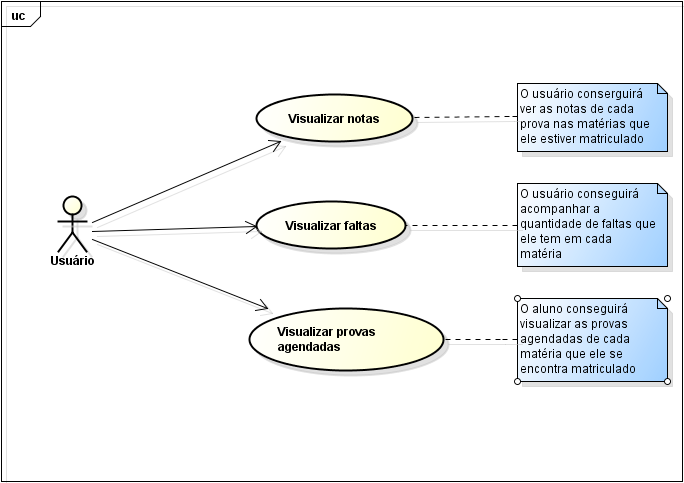
\includegraphics[scale=0.4]{./imagens/2_q_metodologico/qm2.png}}
			\caption[Diagrama de Casos de Uso]{Diagrama de Casos de Uso.
			 \textbf{Fonte:}Elaborado pelos autores.}
			\label{fig:qm2}
		\end{figure}
		
	\par Logo após, foi projetado o diagrama de atividades para se ter uma visão
da sequência do fluxo do sistema, conforme mostra a Figura \ref{fig:qm3}.
		
		
		\begin{figure}[h!]
			\centerline{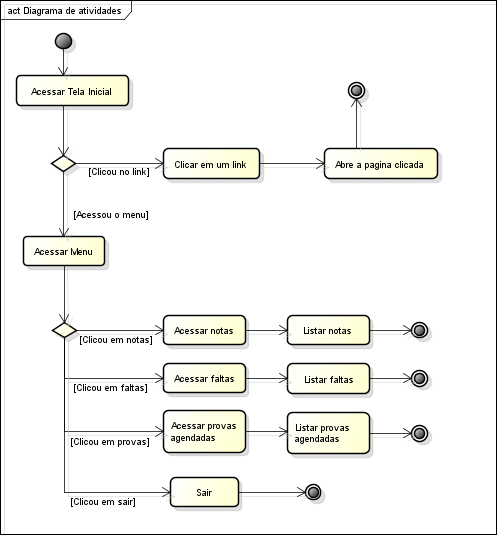
\includegraphics[scale=0.4]{./imagens/2_q_metodologico/qm3.png}}
			\caption[Diagrama de atividades]{Diagrama de atividades.
			 \textbf{Fonte:}Elaborado pelos autores.}
			\label{fig:qm3}
		\end{figure}
		
		\par A próxima etapa realizada foi o desenvolvimento do diagrama de classes do
aplicativo \textit{Android}, o qual tem por objetivo mostrar todas as classes
que o sistema necessita, como pode-se observar na Figura \ref{fig:qm7(1)}.
		
		\pagebreak
		\begin{figure}[h!]
			\centerline{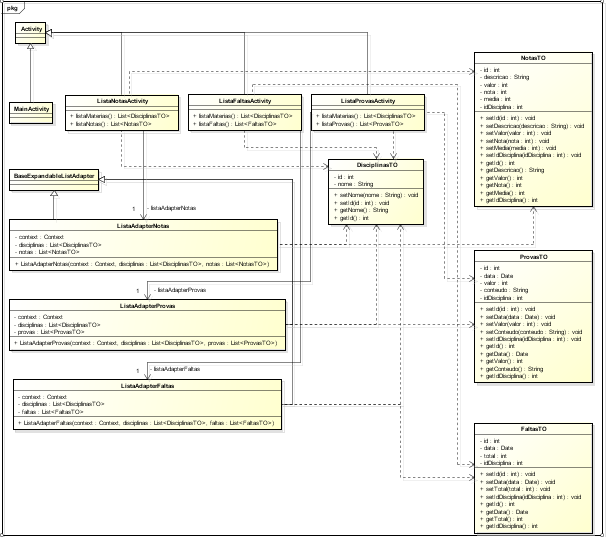
\includegraphics[scale=0.4]{./imagens/2_q_metodologico/qm7(1).png}}
			\caption[Diagrama de classes do aplicativo \textit{Android}]{Diagrama de
			classes do aplicativo \textit{Android}.
			 \textbf{Fonte:}Elaborado pelos autores.}
			\label{fig:qm7(1)}
		\end{figure}